\section{FaisalNajibAbdullah(1174042)}

\subsection{Sejarah}
Sejarah geografi dimulai sejak manusia mulai berinteraksi dengan lingkunganya, hal ini juga merupakan awal mula dari berkembangnya ilmu pengetahuan tentang geografi.
Pada awal dikenalnya sistem informasi geografis bahwa tidak lepas dari adanya kemajuan didalam bidang teknologi. Pada awal tahun 1960 perkembangan sistem informasi geografis dalam ilmu komputer semakin pesat dan siap dingunakan pada bidang milliter. Pada taun 1700 teknik yang digunakan pada survei modern untuk pemetaan topografis digunakan atau diterapkan , hal ini juga termasuk pada versi awal pemetaan tematis.
Pada 35000 tahun yang lalu, di sebuah dinding tepatnya di gua Lascaux, Perancis, para pemburu Cro-Magnon menggambarkan hewan-hewan mangsa mereka. Mereka juga menggambarkan garis-garis yang dipercaya sebagai rute dari migrasi hewan-hewan mangsa mereka tersebut. Catatan awal tersebut sejalan dengan dua elemen struktur pada sistem informasi geografis modern saat ini, arsip grafis yang terhubung ke database atribut. 
Lalu pada tahun 1700-an teknik survei modern untuk pemetaan topografis diterapkan, termasuk versi awal pemetaan tematis, contohnya untuk keilmuan atau data sensus. 
\begin{figure}[H]
	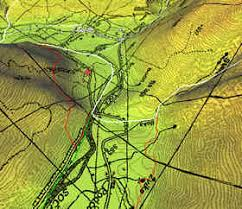
\includegraphics[width=4cm]{figures/1174042/gis.jpg}
	\centering
	\caption{Sejarah Gis}
\end{figure}

\subsection{Link}
\href{https://www.youtube.com/watch?v=8gTLBneTUAo&t=15s}{Youtube}
\subsection{Plagiarism}
\begin{figure}[H]
	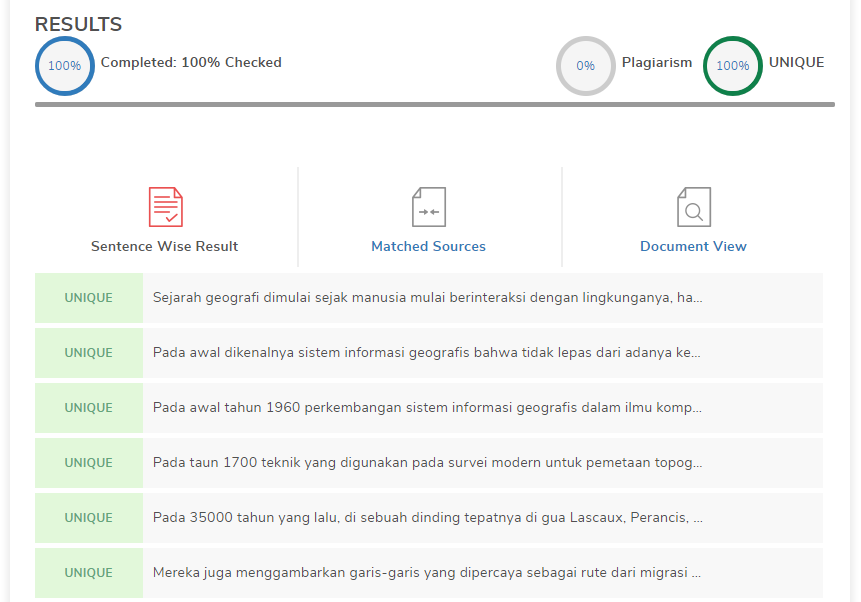
\includegraphics[width=4cm]{figures/1174042/plagiat.png}
	\centering
	\caption{Plagiarism}
\end{figure}